\section{ITERAZIONE 3}

In questa iterazione conclusiva viene sviluppato il secondo modulo algoritmico del
progetto, il \textbf{Predittore Dinamico di Riordino Scorte}, vengono completate
le API di gestione del menù e viene introdotta l'\textbf{autenticazione
dell'amministratore}, che protegge l'accesso al backoffice. L'iterazione si chiude
con il consolidamento della qualità del codice: un intervento di refactoring
guidato da metriche statiche e l'analisi di copertura del backend.

% ============================================================================
\subsection{Casi d'uso implementati}

\begin{table}[H]
\centering
\caption{Casi d'uso sviluppati nell'Iterazione 3}
\label{tab:uc-iter3}
\begin{tabular}{lll}
\toprule
\textbf{ID} & \textbf{Titolo} & \textbf{Relazione} \\
\midrule
UC8 & Autenticazione Admin & definito nell'Iterazione~0 \\
UC9 & Predittore Dinamico di Riordino Scorte & realizza UC5b in forma avanzata \\
\bottomrule
\end{tabular}
\end{table}

Analogamente a quanto fatto nell'Iterazione~2 per lo Smistatore, il modulo del
Predittore riceve un identificatore dedicato (UC9) invece di riusare \texttt{UC5b}.
Il caso d'uso \emph{UC5b -- Aggiornare Scorte}, descritto nell'Iterazione~0 e
implementato nella sua forma base, viene qui realizzato in forma avanzata da UC9:
per non sovraccaricare lo stesso identificatore con due significati distinti tra
iterazioni, il modulo algoritmico è numerato a parte. Il caso d'uso UC8
(Autenticazione Admin) è invece definito a livello di requisiti nell'Iterazione~0
e implementato in questa iterazione.

% ============================================================================
\subsection{Realizzazione dell'autenticazione Admin (UC8)}
L'area di amministrazione (configurazione di
menù, scorte, stampanti e parametri del Predittore) era finora raggiungibile da
chiunque conoscesse l'indirizzo della pagina \texttt{/admin}: viene ora introdotto
un controllo d'accesso dedicato.
\paragraph{Scelte realizzative}\mbox{}\\
La password non viene mai memorizzata in chiaro: nel database è conservato solo il
suo hash \texttt{bcrypt} (con \emph{salt} per-hash e fattore di costo
configurabile), associato all'unico utente con ruolo \texttt{admin} nella tabella
\texttt{utente}, già presente nel modello dati (Figura~\ref{fig:uml_classes_dato}).
Alla verifica positiva il sistema emette un \emph{token di sessione} opaco con
scadenza, che il client presenta nelle richieste successive per accedere alle
funzioni riservate; il token è volatile, quindi un riavvio del server invalida le
sessioni in corso. La password di default impostata dal sistema è \texttt{1111}
(configurabile via variabile d'ambiente al primo avvio) ed è modificabile
dall'Admin dopo l'accesso.

\newpage
\subsection{Diagrammi UML}

Il Predittore Dinamico di Riordino Scorte non introduce nuovi nodi o componenti
nell'architettura: è realizzato come servizio interno al \textit{Web Server}
(modulo \texttt{predittore.js} in \texttt{services/}), invocato sia in modo
periodico sia su evento di vendita, ed esposto verso i client tramite le API REST
descritte più avanti. Per questo motivo i diagrammi UML strutturali di
Deployment e Class per tipo di dato restano quelli presentati nell'Iterazione~2
(Figure~\ref{fig:uml_classes_dato} e~\ref{fig:uml_deployment}). La logica di
funzionamento del modulo è invece dettagliata dal diagramma di flusso in
Figura~\ref{fig:flusso_predittore}.
\\ \\
L'\textbf{autenticazione Admin} (UC8) non incide invece sui diagrammi di
\emph{deployment} né sul modello \emph{dati}, ma aggiunge un componente
all'\textit{Application Logic}. Sul piano dei dati si appoggia interamente alla
classe \texttt{Utente} -- con gli attributi \texttt{password\_hash} e
\texttt{ruolo} -- già presente nel modello dell'Iterazione~2
(Figura~\ref{fig:uml_classes_dato}); non introduce quindi nuove entità né nuovi
nodi di \emph{deployment}, che restano pertanto invariati. Sul piano dei
\emph{componenti}, l'autenticazione è realizzata dal componente
\texttt{GestioneAutenticazione}, interno all'Application Logic, che espone verso
\textit{AdminFrontEnd} l'interfaccia \texttt{AutenticazioneMgmt} (operazioni di
login, verifica, logout e cambio password, corrispondenti agli endpoint
\texttt{/api/auth/admin/*}) e accede alla tabella \texttt{utente} attraverso il
repository dedicato, in linea con la separazione dell'accesso ai dati introdotta
dal refactoring di questa iterazione. La protezione delle funzioni riservate è
affidata al middleware \texttt{richiediAdmin}, che valida il token di sessione e
nega l'accesso con esito \texttt{401} in assenza di token o con ruolo non
amministrativo. Per non rivelare l'esistenza dell'utenza, il login restituisce la
medesima risposta \texttt{401} sia per password errata sia per utente assente; il
token, opaco e con scadenza, è mantenuto in memoria volatile, perciò un riavvio
del server invalida le sessioni in corso.
\\ \\
Per riflettere questa aggiunta, il Component Diagram e il Class Diagram per
interfacce dell'Iterazione~2 sono aggiornati con il componente
\texttt{GestioneAutenticazione} e la relativa interfaccia
\texttt{AutenticazioneMgmt}, come mostrato nelle
Figure~\ref{fig:uml_component_it3} e~\ref{fig:uml_classes_interface_it3}.

\begin{figure}[H]
    \centering
    
\includegraphics[width=\textwidth]{IT3_UML_Component_Diagram.png}
    \caption{UML Component Diagram aggiornato con il componente
             \texttt{GestioneAutenticazione} e l'interfaccia
             \texttt{AutenticazioneMgmt} --- Iterazione~3}
    \label{fig:uml_component_it3}
\end{figure}

\begin{figure}[H]
    \centering
    
\includegraphics[width=\textwidth]{IT3_UML_Class_Diagram_Interface.png}
    \caption{UML Class Diagram per interfacce aggiornato con
             \texttt{AutenticazioneMgmt} --- Iterazione~3}
    \label{fig:uml_classes_interface_it3}
\end{figure}

\newpage
\subsection{Algoritmo: Predittore Dinamico di Riordino Scorte}

\subsubsection*{Introduzione}
L'algoritmo \textbf{Predittore Dinamico di Riordino Scorte} affronta la gestione reattiva delle scorte in sistemi POS per la ristorazione ad alta variabilità (sagre, eventi, locali con picchi imprevisti).

\paragraph{Attori coinvolti}
\begin{itemize}
    \item \textbf{Sistema POS:} emette eventi di vendita e aggiorna i contatori di consumo in tempo reale.
    \item \textbf{Gestore Scorte:} riceve le notifiche di rifornimento suggerito con livello di urgenza.
    \item \textbf{Cassa:} riceve notifiche di blocco per voci con scorta azzerata.
    \item \textbf{Dashboard Admin:} visualizza stato scorte, previsioni di esaurimento e azioni suggerite.
\end{itemize}

\paragraph{Trigger e postcondizioni}
\begin{itemize}
    \item \textbf{Trigger:} Esecuzione periodica (ogni $T$ minuti) oppure event-driven ad ogni vendita registrata.
    \item \textbf{Postcondizione:} Per ogni voce attiva: stima aggiornata del tempo di esaurimento, calcolo dell'indice $U$, e  se $U$ supera la soglia suggerimento di rifornimento con priorità e quantità consigliata.
\end{itemize}

\subsubsection*{Parametri di Input}
Ogni voce attiva viene valutata in base ai parametri della Tabella~\ref{tab:parametri_input}, provenienti dal POS, dal registro vendite e dallo storico rifornimenti.

\begin{table}[htbp]
\centering
\caption{Parametri di Input dell'Algoritmo}
\label{tab:parametri_input}
\small
\begin{tabular}{lp{10cm}}
\toprule
\textbf{Parametro} & \textbf{Descrizione} \\
\midrule
\texttt{quantita\_attuale} & Quantità corrente in scorta, aggiornata ad ogni vendita o rifornimento. \\
\texttt{consumo\_ultimi\_15\_min} & Unità vendute negli ultimi 15 minuti. Cattura i picchi improvvisi. \\
\texttt{consumo\_ultima\_ora} & Unità vendute nell'ultima ora. Trend a medio termine. \\
\texttt{media\_storica\_fascia} & Media storica di vendite nella stessa fascia oraria (da \texttt{scorta\_storico}). \\
\texttt{tempo\_residuo\_evento} & Tempo alla chiusura dell'evento (secondi). Contestualizza l'urgenza. \\
\texttt{tempo\_riapprovvigionamento} & Tempo stimato per completare un rifornimento (secondi). \\
\texttt{priorita\_voce} & Peso nel menu: alta (principali), media, bassa (contorni/extra). \\
\texttt{stato\_scorta} & Flag: disponibile / \texttt{soglia\_giallo} / \texttt{soglia\_rosso} / esaurito. \\
\texttt{ingredienti\_condivisi} & Ingredienti comuni ad altre voci; per il consumo aggregato. \\
\texttt{categoria\_reparto} & Bar, cucina, griglia. Influenza il tempo di riapprovvigionamento. \\
\bottomrule
\end{tabular}
\end{table}

\subsubsection*{Logica di Funzionamento}
Il consumo atteso è una media pesata a tre componenti temporali  comportamento recente, trend a medio termine e baseline storica:

\begin{equation}
\begin{aligned}
\text{consumo\_atteso} ={}& \alpha \cdot \text{consumo\_ultimi\_15\_min} \\
&+ \beta \cdot \text{consumo\_ultima\_ora} \\
&+ \gamma \cdot \text{media\_storica\_stessa\_fascia\_oraria}
\end{aligned}
\end{equation}

con $\alpha + \beta + \gamma = 1$. In condizioni normali: $\alpha = 0.5$, $\beta = 0.3$, $\gamma = 0.2$. In modalità picco ($\text{consumo\_ultimi\_15\_min} > 2 \times \text{media storica}$), $\alpha$ sale fino a $0.8$ e i pesi residui vengono ridistribuiti su $\beta$ e $\gamma$.
\\
Il tempo stimato di esaurimento:
$$ \text{tempo\_esaurimento} = \frac{\text{quantita\_attuale}}{\text{consumo\_atteso}} $$

L'indice di urgenza $U$ quantifica il rischio che la scorta si esaurisca prima del completamento di un rifornimento:
$$ U = \max(0, \text{tempo\_riapprovvigionamento} - \text{tempo\_esaurimento}) \cdot \text{priorita\_voce} $$

$U > 0$ indica che, al ritmo attuale, la scorta si esaurirà prima che il rifornimento possa arrivare. Valori elevati innescano il suggerimento di rifornimento proattivo.

\subsubsection*{Passi dell'Algoritmo}
L'obiettivo è massimizzare il preavviso prima dell'esaurimento di ogni voce.

\begin{enumerate}
    \item[\textbf{Passo 1}] \textbf{Raccolta dati:} Per ogni voce attiva non marcata come ``non vendibile'', il sistema legge: quantità in scorta, contatori di vendita (15 min, 1 ora), fascia oraria corrente per lo storico, metadati di reparto e priorità.

    \item[\textbf{Passo 2}] \textbf{Aggregazione ingredienti condivisi:} Per voci con ingredienti in comune (es.\ patatine condivise tra più piatti), il consumo viene aggregato su tutte le voci collegate, evitando stime divergenti.

    \item[\textbf{Passo 3}] \textbf{Selezione modalità di stima:} Se lo storico per la fascia oraria corrente è assente o insufficiente ($<3$ occorrenze), si attiva la \emph{modalità prudente}: stima basata solo sulle soglie statiche, con $\gamma = 0$.

    \item[\textbf{Passo 4}] \textbf{Rilevamento picco:} Se $\texttt{consumo\_ultimi\_15\_min} > 2\times$ media storica, si attiva la \emph{modalità picco}: $\alpha$ sale a $0.8$ per privilegiare i dati recenti. Flag visivo in dashboard.

    \item[\textbf{Passo 5}] \textbf{Calcolo consumo atteso e tempo di esaurimento:} Si applica la formula ponderata con i coefficienti determinati ai passi precedenti. Se $\text{consumo\_atteso} \le 0$ (nessuna vendita nelle tre finestre), il tempo di esaurimento diventa $\infty$ e la voce è classificata stabile.

    \item[\textbf{Passo 6}] \textbf{Calcolo dell'indice $U$:} $U = \max(0, t_{\text{riapprov}} - t_{\text{esaurimento}}) \times \text{priorità}$. Se $t_{\text{esaurimento}} < t_{\text{residuo\_evento}}$ (la voce si esaurirà prima della chiusura), $U$ riceve un moltiplicatore di contesto aggiuntivo.

    \item[\textbf{Passo 7}] \textbf{Classificazione e notifica:} In base a $U$ e allo stato della scorta (Tabella~\ref{tab:classificazione_notifica}), il sistema classifica la voce e, se necessario, genera un suggerimento di rifornimento. Quantità suggerita: $\lceil \text{consumo\_atteso} \times t_{\text{riapprov}} \times 1.3 \rceil$.

    \item[\textbf{Passo 8}] \textbf{Loop e aggiornamento:} Completato il ciclo su tutte le voci, il sistema attende il prossimo tick ($T$ minuti) o la prossima vendita. Le stime vengono ricalcolate integralmente ad ogni esecuzione.
\end{enumerate}

\begin{table}[htbp]
\centering
\caption{Classificazione delle Voci e Azioni Conseguenti}
\label{tab:classificazione_notifica}
\small
\begin{tabularx}{\textwidth}{l>{\raggedright\arraybackslash}X>{\raggedright\arraybackslash}X}
\toprule
\textbf{Classificazione} & \textbf{Condizione} & \textbf{Azione} \\
\midrule
Stabile & $U = 0$ e scorta disponibile & Nessuna azione. Monitoraggio continuativo. \\
Attenzione & $0 < U \le \text{soglia\_warn}$ & Notifica informativa in dashboard. \\
Urgente & $U > \text{soglia\_warn}$ e scorta $\neq$ esaurita & Suggerimento di rifornimento prioritario. Alert visivo. \\
Critico / Esaurito & $\texttt{quantita\_attuale} = 0$ & Voce non vendibile. Notifica cassa. Richiesta conferma. \\
\bottomrule
\end{tabularx}
\end{table}

\subsubsection*{Casi Limite e Comportamenti Attesi}

\begin{table}[htbp]
\centering
\caption{Gestione dei Casi Limite}
\label{tab:casi_limite}
\small
\begin{tabularx}{\textwidth}{l>{\raggedright\arraybackslash}X>{\raggedright\arraybackslash}X}
\toprule
\textbf{Caso limite} & \textbf{Condizione} & \textbf{Comportamento} \\
\midrule
Storico assente & Nessun dato in \texttt{scorta\_storico}. & Modalità prudente: solo soglie statiche, $\gamma = 0$. Notifica admin. \\
Picco improvviso & $\text{consumo\_15min} > 2\times \text{media storica}$. & $\alpha$ a $0.8$. Flag picco in dashboard. Ricalcolo immediato di $U$. \\
Scorta azzerata & $\texttt{quantita\_attuale} = 0$. & Voce non vendibile. Notifica cassa. Riattivazione solo con conferma. \\
Consumo nullo & Nessuna vendita nelle 3 finestre. & $t_{\text{esaurimento}} = \infty$. Voce stabile. \\
Ingredienti condivisi & Più voci usano lo stesso ingrediente. & Consumo aggregato. Unico indice $U$ per l'ingrediente. \\
Tempo residuo $<$ riapprov. & Evento finisce prima del rifornimento. & $U$ moltiplicato per fattore contesto. Alert immediato se urgente. \\
Reparto offline & Nessun aggiornamento dal reparto. & Ultimo consumo noto mantenuto. Warning staleness. Modalità prudente. \\
\bottomrule
\end{tabularx}
\end{table}

\subsubsection*{Analisi di Complessità}
Siano $n$ il numero di voci attive, $h$ il numero di voci in storico per fascia oraria, $s$ il numero medio di ingredienti condivisi per voce.

\begin{table}[htbp]
\centering
\caption{Complessità Computazionale}
\label{tab:complessita_predittore}
\small
\begin{tabular}{ll}
\toprule
\textbf{Fase} & \textbf{Complessità} \\
\midrule
Lettura dati per voce & $\mathcal{O}(n)$ \\
Aggregazione ingredienti condivisi & $\mathcal{O}(n \cdot s)$ \\
Recupero storico fascia oraria & $\mathcal{O}(n \cdot h)$ \\
Calcolo \texttt{consumo\_atteso}, $t_{\text{esaurimento}}$, $U$ & $\mathcal{O}(1)$ per voce \\
Classificazione e notifica & $\mathcal{O}(1)$ per voce \\
\midrule
\textbf{Totale per ciclo} & $\mathbf{\mathcal{O}(n \cdot (h + s))}$ \\
\bottomrule
\end{tabular}
\end{table}

Con $n \le 200$, $h \le 50$, $s \le 5$, l'algoritmo è adatto all'esecuzione in tempo reale con latenza trascurabile.

\subsubsection*{Pseudocodice}

\begin{algorithm}[H]
\caption{Procedura principale PredictReorder}
\label{alg:predict_reorder}
\begin{algorithmic}[1]
\Procedure{PredictReorder}{$menu\_items, storico, now$} \Comment{$\mathcal{O}(n \cdot (h + s))$}
    \For{each $voce \in menu\_items$} \Comment{$\mathcal{O}(n)$}
        \If{$voce.stato = \text{'non\_vendibile'}$}
            \State \textbf{continue}
        \EndIf
        \State $consumo \gets \Call{AggregaConsumo}{voce, menu\_items}$ \Comment{$\mathcal{O}(s)$}
        \If{$\Call{StoricoDisponibile}{voce, now}$} \Comment{$\mathcal{O}(h)$}
            \State $\alpha, \beta, \gamma \gets \Call{CalcolaPesi}{voce, consumo}$ \Comment{$\mathcal{O}(1)$}
        \Else
            \State $\alpha, \beta, \gamma \gets \text{MODALITA\_PRUDENTE}$ \Comment{soglie statiche}
        \EndIf
        \State $c\_atteso \gets \alpha \cdot consumo.ultimi\_15 + \beta \cdot consumo.ultima\_ora + \gamma \cdot \Call{StoriciFascia}{voce, now}$ \Comment{$\mathcal{O}(1)$}
        \If{$c\_atteso \le 0$}
            \State $voce.t\_esaurimento \gets \infty$
            \State $voce.classe \gets \text{STABILE}$
            \State \textbf{continue}
        \EndIf
        \State $voce.t\_esaurimento \gets voce.q\_attuale / c\_atteso$ \Comment{$\mathcal{O}(1)$}
        \State $voce.U \gets \max(0, voce.t\_riapprov - voce.t\_esaurimento) \cdot voce.priorita$ \Comment{$\mathcal{O}(1)$}
        \State $voce.classe \gets \Call{Classifica}{voce}$ \Comment{$\mathcal{O}(1)$}
        \If{$voce.classe \in \{\text{URGENTE}, \text{CRITICO}\}$}
            \State $q\_sug \gets \lceil c\_atteso \cdot voce.t\_riapprov \cdot \text{SAFETY} \rceil$ \Comment{$\mathcal{O}(1)$}
            \State \Call{GeneraNotifica}{$voce, q\_sug$} \Comment{$\mathcal{O}(1)$}
        \EndIf
    \EndFor
\EndProcedure
\end{algorithmic}
\end{algorithm}

\begin{algorithm}[H]
\caption{Funzioni ausiliarie}
\label{alg:funzioni_ausiliarie}
\begin{algorithmic}[1]
\Procedure{AggregaConsumo}{$voce, menu\_items$} \Comment{$\mathcal{O}(s)$}
    \State $c \gets voce.consumo\_raw$
    \For{each $ing \in voce.ingredienti\_condivisi$}
        \For{each $altra \in menu\_items$}
            \If{$ing \in altra.ingredienti$}
                \State $c \gets c + altra.consumo\_raw$
            \EndIf
        \EndFor
    \EndFor
    \State \Return $c$
\EndProcedure

\medskip

\Procedure{CalcolaPesi}{$voce, consumo$} \Comment{$\mathcal{O}(1)$}
    \If{$consumo.ultimi\_15 > 2.0 \times \Call{StoriciFascia}{voce, now}$}
        \State \Return $\alpha=0.8, \beta=0.15, \gamma=0.05$ \Comment{modalità picco}
    \Else
        \State \Return $\alpha=0.5, \beta=0.30, \gamma=0.20$ \Comment{modalità normale}
    \EndIf
\EndProcedure

\medskip

\Procedure{Classifica}{$voce$} \Comment{$\mathcal{O}(1)$}
    \If{$voce.q\_attuale = 0$} \Return $\text{CRITICO}$ \EndIf
    \If{$voce.U = 0$} \Return $\text{STABILE}$ \EndIf
    \If{$voce.U \le \text{SOGLIA\_WARN}$} \Return $\text{ATTENZIONE}$ \EndIf
    \State \Return $\text{URGENTE}$
\EndProcedure
\end{algorithmic}
\end{algorithm}

\subsubsection*{Note Implementative}
\begin{itemize}
    \item \textbf{Configurazione:} $\alpha$, $\beta$, $\gamma$, $\text{SOGLIA\_WARN}$ e $\text{SAFETY}$ sono configurabili per evento/locale via pannello admin. Default: $\text{SOGLIA\_WARN} = 300$\,s, $\text{SAFETY} = 1.3$, tick $T = 5$\,min.
    \item \textbf{Persistenza:} i contatori a 15 min e 1 ora sono in memoria volatile ad alta frequenza. Lo storico multi-evento viene scritto su \texttt{scorta\_storico} a fine evento per alimentare le previsioni future.
    \item \textbf{Integrazione con UC7:} il Predittore può essere invocato dallo Smistatore Intelligente prima del routing, bloccando in anticipo l'assegnazione di task per voci CRITICO ed evitando comande non evadibili.
\end{itemize}

\clearpage
\begin{figure}[H]
    \centering
    
\includegraphics[height=0.90\textheight, keepaspectratio]{predittore_flusso.drawio.png}
    \caption{Diagramma di flusso  Predittore Dinamico di Riordino Scorte}
    \label{fig:flusso_predittore}
\end{figure}

\clearpage
% ============================================================================
%  BLOCCO TEST (struttura in stile OptiTour:
%  analisi statica/refactoring -> test automatizzati -> copertura -> API)
% ============================================================================

\definecolor{refPrima}{HTML}{D45454} % rosso = prima del refactoring
\definecolor{refDopo}{HTML}{5BA85E}  % verde = dopo il refactoring

% Stile comune ai tre grafici a barre orizzontali raggruppate
\pgfplotsset{
    refbar/.style={
        xbar,
        width=\linewidth,
        bar width=7pt,
        enlarge y limits=0.2,
        xmin=0,
        axis x line*=bottom,
        axis y line*=left,
        ytick=data,
        nodes near coords,
        nodes near coords align={horizontal},
        every node near coord/.append style={font=\scriptsize},
        legend style={at={(0.97,0.05)}, anchor=south east, font=\small, draw=none},
        legend cell align={left},
        tick label style={font=\small},
        xlabel style={font=\small},
    }
}



\subsection{Test}

% -
\subsubsection{Analisi statica del codice e refactoring}

Il codice è stato sottoposto a un intervento di refactoring guidato da metriche
statiche: la complessità ciclomatica delle funzioni (misurata con ESLint),
l'accoppiamento tra moduli e le dipendenze circolari (analizzati con madge) e la
dimensione dei moduli in righe di codice. L'obiettivo non era aggiungere
funzionalità, ma rendere il codice più semplice da leggere e da mantenere
riducendo la complessità delle funzioni più critiche e l'accoppiamento verso il
database.

\paragraph{Interventi sul backend}\mbox{}\\

\subparagraph{Separazione dell'accesso ai dati.}
Nella versione iniziale le query SQL erano scritte direttamente all'interno dei
gestori delle route, mescolando in uno stesso file la logica HTTP, l'accesso al
database e la costruzione delle risposte. Le query sono state spostate in un
layer dedicato (la cartella \texttt{repositories/}), con un unico punto di
accesso al pool di connessioni. In questo modo le route delegano la persistenza
ai repository e non conoscono più il dettaglio delle tabelle. Il numero di
moduli che dipendono direttamente da \texttt{db.js} passa da 10 a 2 (si veda la
Figura~\ref{fig:ref-accoppiamento}), e la stessa estrazione ha permesso di
alleggerire i gestori che prima contenevano le query.

\subparagraph{Sottosistema di stampa dietro una façade.}
La catena che porta dall'ordine confermato alla stampa (smistatore, formatter,
dispatcher ed emulatore ESC/POS) era invocata direttamente dalle route, che
quindi dipendevano da quattro servizi distinti. È stata incapsulata dietro una
\emph{façade} (\texttt{services/stampa/}) che espone poche operazioni di alto
livello: le route ora dipendono da un solo modulo. Contestualmente il dispatcher
e l'emulatore non accedono più al database in modo diretto ma tramite i
repository, riducendo ulteriormente l'accoppiamento.

\subparagraph{Riduzione della complessità.}
Le due funzioni più complesse del backend sono state ristrutturate. Il parser
del flusso ESC/POS (\texttt{parsaFlusso}), costituito da un unico ciclo con una
lunga catena di condizioni sui codici di comando, è stato riscritto con una
tabella di dispatch che associa a ogni comando una piccola funzione dedicata: la
complessità ciclomatica scende da 51 a 11. La funzione di predizione delle
scorte (\texttt{eseguiPredizione}) è stata scomposta in funzioni pure più piccole
(la valutazione della singola voce e la derivazione dello stato di scorta),
passando da 21 a 2.

\paragraph{Interventi sul frontend}\mbox{}\\
I due componenti principali dell'interfaccia, \texttt{Admin.jsx} e
\texttt{Cassa.jsx}, concentravano in un unico file lo stato, la logica, le
chiamate al backend e numerose finestre modali: rispettivamente 1489 e 742 righe.
Sono stati scomposti in circa venti tra componenti e hook a responsabilità
singola, introducendo un client centralizzato per le chiamate API ed estraendo
in funzioni separate la validazione dei dati e la costruzione dei payload. La
dimensione di \texttt{Admin.jsx} scende da 1328 a 150 righe di codice e quella di
\texttt{Cassa.jsx} da 669 a 227 (Figura~\ref{fig:ref-coesione}).

\paragraph{Risultati}\mbox{}\\
I tre grafici seguenti confrontano le metriche prima e dopo il refactoring.

%  Grafico 1: complessità ciclomatica delle funzioni critiche -
\begin{figure}[ht]
    \centering
    \resizebox{\textwidth}{!}{%
    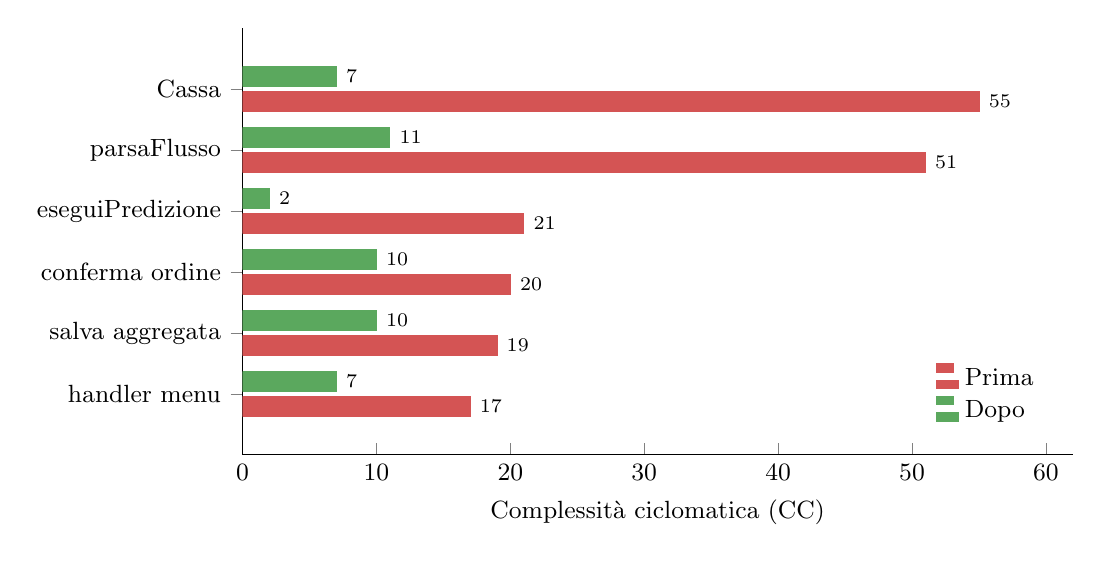
\begin{tikzpicture}
        \begin{axis}[refbar,
            height=7cm, xmax=62,
            xlabel={Complessità ciclomatica (CC)},
            symbolic y coords={f1,f2,f3,f4,f5,f6},
            yticklabels={handler menu, salva aggregata, conferma ordine,
                         eseguiPredizione, parsaFlusso, Cassa},
        ]
            \addplot[fill=refPrima, draw=refPrima] coordinates {
                (17,f1) (19,f2) (20,f3) (21,f4) (51,f5) (55,f6)};
            \addplot[fill=refDopo, draw=refDopo] coordinates {
                (7,f1) (10,f2) (10,f3) (2,f4) (11,f5) (7,f6)};
            \legend{Prima, Dopo}
        \end{axis}
    \end{tikzpicture}%
    }
    \caption{Complessità ciclomatica delle funzioni più critiche}
    \label{fig:ref-complessita}
\end{figure}

%  Grafico 2: accoppiamento 
\begin{figure}[ht]
    \centering
    \resizebox{\textwidth}{!}{%
    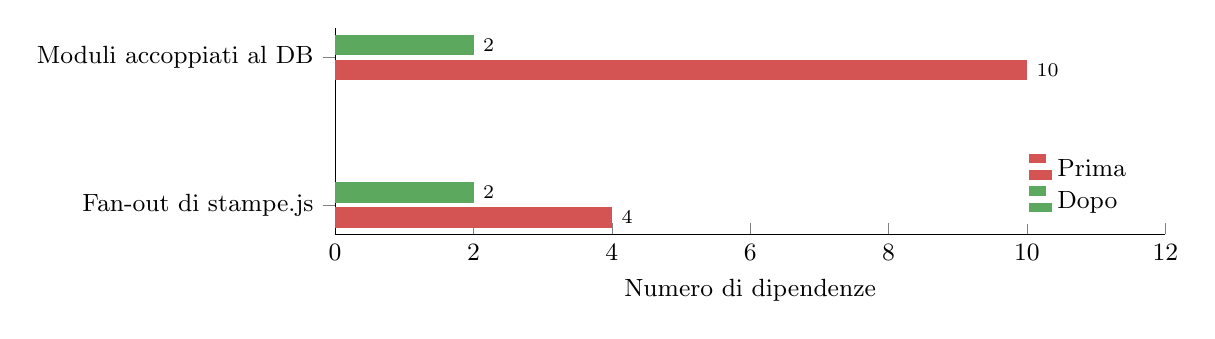
\begin{tikzpicture}
        \begin{axis}[refbar,
            height=4.2cm, xmax=12,
            xlabel={Numero di dipendenze},
            symbolic y coords={a1,a2},
            yticklabels={Fan-out di stampe.js, Moduli accoppiati al DB},
        ]
            \addplot[fill=refPrima, draw=refPrima] coordinates {(4,a1) (10,a2)};
            \addplot[fill=refDopo, draw=refDopo] coordinates {(2,a1) (2,a2)};
            \legend{Prima, Dopo}
        \end{axis}
    \end{tikzpicture}%
    }
    \caption{Accoppiamento prima e dopo.}
    \label{fig:ref-accoppiamento}
\end{figure}

%  Grafico 3: coesione (dimensione dei moduli) --
\begin{figure}[H]
    \centering
    \resizebox{\textwidth}{!}{%
    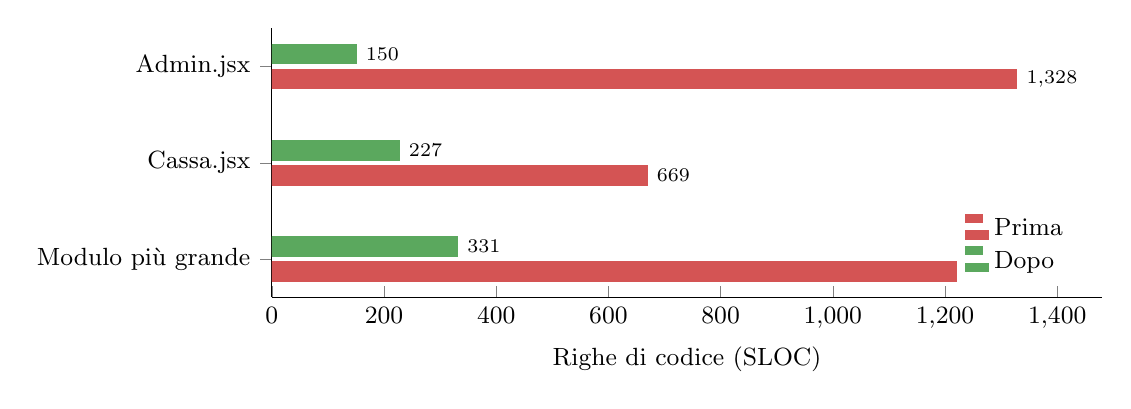
\begin{tikzpicture}
        \begin{axis}[refbar,
            height=5cm, xmax=1480,
            xlabel={Righe di codice (SLOC)},
            symbolic y coords={c1,c2,c3},
            yticklabels={Modulo più grande, Cassa.jsx, Admin.jsx},
        ]
            \addplot[fill=refPrima, draw=refPrima] coordinates {(1328,c1) (669,c2) (1328,c3)};
            \addplot[fill=refDopo, draw=refDopo] coordinates {(331,c1) (227,c2) (150,c3)};
            \legend{Prima, Dopo}
        \end{axis}
    \end{tikzpicture}%
    }
    \caption{Coesione vista come decomposizione dei moduli: i due ``God
    Component'' del frontend e il modulo più grande del progetto vengono divisi
    in unità a responsabilità singola.}
    \label{fig:ref-coesione}
\end{figure}

%  Tabella riepilogativa 
\begin{table}[H]
    \centering
    \begin{tabular}{lcc}
        \hline
        \textbf{Metrica} & \textbf{Prima} & \textbf{Dopo} \\
        \hline
        Funzioni con complessità ciclomatica ${}>{}$ 15 & 11 & 5 \\
        Complessità ciclomatica massima                  & 55 & 37 \\
        Moduli accoppiati al DB ($C_a$ di \texttt{db.js}) & 10 & 2 \\
        Dipendenze circolari                              & 0  & 0 \\
        Modulo più grande (righe di codice)               & 1328 & 331 \\
        Numero di moduli                                  & 19 & 50 \\
        \hline
    \end{tabular}
    \caption{Sintesi delle metriche prima e dopo il refactoring.}
    \label{tab:ref-metriche}
\end{table}

\newpage 
\subsubsection{Test automatizzati}

Come per lo Smistatore, il Predittore è coperto da una suite di test automatizzati
con \textbf{Vitest}

\begin{figure}[H]
    \centering
    
\includegraphics[width=0.92\textwidth]{IT3_test_predittore.png}
    \caption{Esecuzione della suite unitaria del Predittore con Vitest:
             33/33 test unitari superati.}
    \label{fig:test-predittore}
\end{figure}

I test unitari sono organizzati per funzione interna dell'algoritmo:

\begin{enumerate}
    \item \textbf{Selezione della modalità} (\texttt{calcolaPesi}). Verificano la
    scelta tra le modalità \emph{normale}, \emph{picco} e \emph{prudente}  con i
    pesi $\alpha$, $\beta$, $\gamma$ che sommano sempre a 1  e la corretta
    gestione del caso di storico nullo, senza divisioni per zero.

    \item \textbf{Consumo atteso e tempo di esaurimento} (\texttt{consumoAtteso},
    \texttt{tempoEsaurimentoSec}). Validano la media pesata a tre componenti
    temporali e il calcolo del tempo di esaurimento, che con consumo nullo o
    negativo deve restituire $\infty$.

    \item \textbf{Indice di urgenza $U$} (\texttt{calcolaU}). Verificano l'effetto
    dei moltiplicatori di priorità (alta 1.5, media 1.0, bassa 0.5) e del
    moltiplicatore di contesto evento (1.2), oltre al caso $U = 0$ quando la scorta
    si esaurisce dopo il completamento del rifornimento.

    \item \textbf{Classificazione} (\texttt{classifica}). Validano l'assegnazione
    dei quattro stati \emph{esaurito}, \emph{stabile}, \emph{attenzione} e
    \emph{urgente} in base a $U$ e allo stato della scorta.

    \item \textbf{Quantità suggerita e aggregazioni} (\texttt{quantitaSuggerita},
    \texttt{aggregaConsumiCondivisi}, \texttt{tempoResiduoEventoSec}). Coprono la
    formula $\lceil \text{consumo} \cdot t_{riapp} \cdot 1.3 \rceil$, il consumo
    aggregato tra voci con ingredienti condivisi e il calcolo del tempo residuo
    dell'evento.
\end{enumerate}

% -

\subsubsection*{Test autenticazione Admin}

L'autenticazione Admin (UC8) è coperta da una suite \textbf{Vitest} dedicata,
articolata come per gli altri moduli in \textbf{test unitari} sulle funzioni pure
del servizio di autenticazione e \textbf{test di integrazione HTTP} sugli endpoint. L'esito complessivo della suite è riportato in Figura~\ref{fig:test-auth-runner}.

I \textbf{test unitari} (file \texttt{\_\_tests\_\_/auth.test.js}) verificano in
isolamento dal database:
\begin{enumerate}
    \item \textbf{Verifica password} (\texttt{hashPassword}, \texttt{verificaPassword}):
    l'hash prodotto è in formato \texttt{bcrypt} e non in chiaro; la verifica
    restituisce \emph{vero} solo con la password corretta e \emph{falso} (senza
    sollevare eccezioni) con password errata o hash assente/malformato.
    \item \textbf{Ciclo di vita del token} (\texttt{creaToken},
    \texttt{validaToken}, \texttt{revocaToken}): emissione di un token con scadenza
    futura, riconoscimento di un token valido, rifiuto di token inesistenti,
    scaduti (con rimozione automatica) o revocati dopo il logout.
    \item \textbf{Estrazione del token} (\texttt{estraiToken}): lettura del token
    dall'header \texttt{Authorization: Bearer} e gestione dei casi di header
    assente o con formato errato.
    \item \textbf{Middleware di protezione} (\texttt{richiediAdmin}): accesso
    consentito con token admin valido, negato con esito \texttt{401} in assenza di
    token o con token di ruolo non amministrativo.
\end{enumerate}

I \textbf{test di integrazione HTTP} (file
\texttt{\_\_tests\_\_/auth-integrazione.test.js}) validano end-to-end il flusso
sugli endpoint reali: login con password corretta (\texttt{200} con token), login
con password errata (\texttt{401}) o assente (\texttt{400}), verifica del token,
protezione delle operazioni riservate in assenza di token (\texttt{401}), logout
con invalidazione del token e cambio password con successivo ripristino del valore
di default per garantire l'idempotenza tra esecuzioni.

\begin{figure}[H]
    \centering
    
\includegraphics[width=0.95\textwidth]{IT3_test_auth.png}
    \caption{Esecuzione della suite di autenticazione Admin con Vitest}
    \label{fig:test-auth-runner}
\end{figure}

% -

\subsubsection{Analisi di copertura del backend}

\paragraph{Validazione con Vitest}\mbox{}\\
La copertura del codice è misurata con il provider \texttt{v8} di Vitest, configurato per analizzare i moduli algoritmici in \texttt{services/} (\texttt{predittore.js} e \texttt{smistatore.js}). I test che la esercitano comprendono sia i test unitari sia i test di integrazione HTTP eseguiti in ambiente Docker, già descritti nelle sezioni \emph{Test automatizzati} delle Iterazioni~2 e~3.

\subparagraph{Struttura della suite.}
Le suite dei due moduli algoritmici comprendono complessivamente \textbf{71 test} distribuiti su 4 file (di cui \textbf{59 test unitari} e \textbf{12 test di integrazione}); a queste si aggiungono i \textbf{23 test} dell'autenticazione Admin (si veda la sezione \emph{Test dell'autenticazione Admin}), per un totale di \textbf{94 test} su 6 file. Le metriche di copertura riportate di seguito si riferiscono specificamente ai due moduli algoritmici \texttt{predittore.js} e \texttt{smistatore.js}, sui quali è configurato il provider di copertura.

\subparagraph{Setup dei test di integrazione.}
Ogni test di integrazione verifica un flusso end-to-end reale: la richiesta HTTP attraversa il router Express, attiva la logica di business (smistatore o predittore), interagisce con il database MySQL/MariaDB e, ove previsto, pilota gli emulatori di stampa.

Per garantire l'\emph{idempotenza} tra esecuzioni successive, ogni test è preceduto da una fase di \texttt{beforeEach} che:
\begin{enumerate}
    \item riaccende tutte le stampanti emulate
          (\texttt{POST /api/stampe/emulatore/:id/accendi});
    \item ripristina le scorte delle voci utilizzate nei test
          a quantità elevate tramite
          \texttt{PUT /api/scorte/:voce\_id};
    \item drena le code interne dello smistatore
          (\texttt{POST /api/smistatore/completa}) per annullare
          il carico residuo di esecuzioni precedenti.
\end{enumerate}

\subparagraph{Casi di test di integrazione.}

\begin{table}[H]
    \centering
    \caption{Test di integrazione HTTP eseguiti con backend Docker attivo.}
    \label{tab:test-integrazione}
    \small
    \begin{tabular}{p{0.20\linewidth}p{0.52\linewidth}p{0.18\linewidth}}
        \toprule
        \textbf{Modulo} & \textbf{Caso di test} & \textbf{Verifica} \\
        \midrule
        \multirow{5}{*}{\texttt{smistatore}}
        & \texttt{GET /api/stampanti} restituisce almeno 4 stampanti
        & Configurazione DB \\
        & Ordine multi-reparto $\to$ comande corrette + audit OK
        & Routing + stampa \\
        & Stampante spenta + ordine cucina $\to$ routing su \texttt{cucina\_2}
        & Fallback dinamico \\
        & Ordine asporto $\to$ $P_{\text{asporto}} > P_{\text{tavolo}}$
          con $\Delta P \geq 40$
        & Bonus priorità~$B$ \\
        & Scorta esaurita $\to$ riga in \texttt{bloccati},
          le altre proseguono
        & Guardia scorte \\
        \midrule
        \multirow{7}{*}{\texttt{predittore}}
        & \texttt{GET /api/predittore/scorte} ritorna lista voci con tutti i campi
        & Schema risposta \\
        & Filtro \texttt{?stato=stabile} restituisce solo voci stabili
        & Query filtering \\
        & \texttt{GET /api/predittore/configurazione} ritorna i 3 parametri
        & Lettura config \\
        & \texttt{PUT .../configurazione/:k} aggiorna e persiste il valore
        & Scrittura config \\
        & Voce con quantità${}=0$ $\to$ stato \texttt{"esaurito"}
        & Classificazione \\
        & Voce senza consumo recente $\to$ \texttt{tempo\_esaurimento = null}
        & Caso limite \\
        & Conteggi coerenti con il totale delle predizioni
        & Integrità dati \\
        \bottomrule
    \end{tabular}
\end{table}


\begin{figure}[H]
    \centering
    
\includegraphics[width=\linewidth]{IT2_end_to_end_copertura.PNG}
    \caption{Esecuzione completa della suite Vitest con Docker attivo
             e report di copertura: 71/71 test superati (4~file,
             nessuno saltato), copertura globale al 94{,}4\%
             di branch (100\% su statement, funzioni e righe).}
    \label{fig:vitest-docker-coverage}
\end{figure}

La copertura globale si attesta al 94{,}4\% di branch perché il provider \texttt{v8} di Vitest è configurato per misurare i soli moduli in \texttt{services/} (\texttt{predittore.js} e \texttt{smistatore.js}): i rami aggiuntivi esercitati dai test di integrazione ricadono infatti in \texttt{routes/} e \texttt{repositories/}, che si trovano al di fuori del perimetro misurato.
\\ \\
Questi test restano comunque essenziali, perché verificano l'intera catena \emph{HTTP $\to$ router $\to$ service $\to$ repository $\to$ database $\to$ emulatore di stampa} in condizioni realistiche (errori di rete, latenza TCP, stato persistente, concorrenza tra stampanti) non raggiungibili o verificabili dai soli test unitari.

\subsubsection{API esposte}

Gli endpoint seguenti supportano il Predittore, realizzano l'autenticazione Admin
e completano la gestione del menù; valgono le convenzioni REST definite
nell'Iterazione~1. Le operazioni di
scrittura (\POST, \PUT) sono verificate tramite Postman, di cui si riporta
richiesta e risposta.

% ─────────────────────────────────────────────────────────────────────────────
\paragraph{Predittore}\mbox{}\\

Espone le previsioni di esaurimento scorte calcolate dal \textbf{Predittore
Dinamico di Riordino Scorte} (UC9) e permette di configurarne i parametri
a runtime.

\apicall{\GET~\texttt{/api/predittore/scorte}}

Esegue il ciclo di predizione su tutte le voci attive e restituisce le
previsioni ordinate per indice di urgenza $U$ decrescente. Supporta due
parametri opzionali di filtro:
\begin{itemize}
  \item \texttt{?stato=urgente,esaurito}  filtra per stato (CSV);
  \item \texttt{?reparto=cucina}  filtra per reparto di stampa.
\end{itemize}

\begin{lstlisting}[style=json]
{
  "generato_a": "2026-05-26T20:20:00.000Z",
  "configurazione": { "evento_fine_oggi": "23:30",
                      "soglia_warn_urgenza": "300",
                      "giorni_storico": "30" },
  "conteggi": { "totale": 12, "stabile": 8,
                "attenzione": 2, "urgente": 1, "esaurito": 1 },
  "predizioni": [
    { "voce_id": 2, "nome": "Polenta taragna", "stato": "urgente",
      "U": 520.0, "quantita_attuale": 4,
      "tempo_esaurimento_min": 18, "quantita_suggerita": 30,
      "reparto": "cucina" }
  ]
}
\end{lstlisting}

\apicall{\GET~\texttt{/api/predittore/scorte/:voce\_id}}

Predizione dettagliata per una singola voce. Risposta 404 se la voce non
esiste o non ha la gestione scorte attiva.

\begin{lstlisting}[style=json]
{ "voce_id": 2, "nome": "Polenta taragna", "stato": "urgente",
  "U": 520.0, "quantita_attuale": 4,
  "consumo_atteso": 2.1, "tempo_esaurimento_min": 18,
  "quantita_suggerita": 30, "reparto": "cucina",
  "modalita": "normale" }
\end{lstlisting}

\apicall{\GET~\texttt{/api/predittore/configurazione}}

Restituisce la configurazione corrente del predittore dalla tabella
\texttt{configurazione}.

\begin{lstlisting}[style=json]
{
  "evento_fine_oggi":   "23:30",
  "soglia_warn_urgenza": "300",
  "giorni_storico":      "30"
}
\end{lstlisting}

\apicall{\PUT~\texttt{/api/predittore/configurazione/:chiave}}

Aggiorna o crea (upsert) un singolo parametro di configurazione del predittore.
Campo obbligatorio: \texttt{valore}.

\postman{i3-pred-config-put.png}{Postman --- \texttt{PUT /api/predittore/configurazione/:chiave}}

\apicall{\PUT~\texttt{/api/predittore/voce/:id}}

Aggiorna i parametri di previsione specifici di una voce: tempo di
riapprovvigionamento (secondi) e/o priorità (\texttt{bassa}, \texttt{media},
\texttt{alta}). Almeno un campo deve essere presente.

\postman{i3-pred-voce-put.png}{Postman --- \texttt{PUT /api/predittore/voce/:id}}

% ─────────────────────────────────────────────────────────────────────────────
\paragraph{Menu  endpoint aggiuntivi}\mbox{}\\

Completano la documentazione API del Menu dell'Iterazione~1 con le funzionalità
di gestione settori, pietanze aggregate, allergeni e opzioni di configurazione,
a supporto dei componenti \texttt{GestioneAllergeni} e
\texttt{GestioneConfigurazione} introdotti nell'architettura dell'Iterazione~2.

\apicall{\GET~\texttt{/api/menu/settori}}

Restituisce la lista distinta dei settori di visualizzazione con il conteggio
delle voci e il colore dominante del settore.

\begin{lstlisting}[style=json]
[
  { "settore_visualizzazione": "Bar",    "num_pietanze": 6, "colore": "#2980B9" },
  { "settore_visualizzazione": "Primi",  "num_pietanze": 6, "colore": "#E8A838" }
]
\end{lstlisting}

\apicall{\GET~\texttt{/api/menu/opzioni}}

Restituisce i valori distinti dei campi usati nei dropdown del pannello Admin
(categorie, settori di stampa, settori di visualizzazione).

\begin{lstlisting}[style=json]
{
  "categorie":               ["Bevanda", "Contorno", "Dolce", "Primo", "Secondo"],
  "settori_stampa":          ["bar", "cucina", "griglia"],
  "settori_visualizzazione": ["Bar", "Contorni", "Dolci", "Primi", "Secondi"]
}
\end{lstlisting}

\apicall{\GET~\texttt{/api/menu/tutti-allergeni}}

Restituisce una mappa \texttt{voce\_id} $\to$ lista allergeni per \emph{tutte}
le voci del menu in un'unica chiamata. Usato dalla cassa per il precarico
all'avvio, evitando richieste individuali per ogni prodotto.

\begin{lstlisting}[style=json]
{
  "3":  [{ "id": 1, "nome": "Glutine",  "descr": "Cereali contenenti glutine" },
         { "id": 4, "nome": "Uova",     "descr": "Uova e derivati"             }],
  "16": [{ "id": 5, "nome": "Solfiti",  "descr": "Anidride solforosa e solfiti"}]
}
\end{lstlisting}

\apicall{\GET~\texttt{/api/menu/:id/allergeni}}

Allergeni associati a una singola voce. Risposta 200 con array vuoto se nessun
allergene è registrato per quella voce.

\begin{lstlisting}[style=json]
[
  { "id": 1, "nome": "Glutine", "descr": "Cereali contenenti glutine" },
  { "id": 4, "nome": "Uova",   "descr": "Uova e derivati"             }
]
\end{lstlisting}

\apicall{\GET~\texttt{/api/menu/:id/composizione}}

Restituisce i componenti di una pietanza aggregata (es.\ menu fisso composto da
più voci singole). Array vuoto se la voce non è aggregata.

\begin{lstlisting}[style=json]
[
  { "id": 1, "codice": "P001", "nome": "Risotto ai funghi",
    "prezzo": "9.00", "categoria": "Primo",
    "settore_visualizzazione": "Primi" },
  { "id": 7, "codice": "S001", "nome": "Costine alla griglia",
    "prezzo": "12.00", "categoria": "Secondo",
    "settore_visualizzazione": "Secondi" }
]
\end{lstlisting}

\apicall{\POST~\texttt{/api/menu/aggregata}}

Crea una pietanza aggregata composta da più voci esistenti. Il codice è
auto-generato come per \texttt{POST /api/menu}. Campi obbligatori:
\texttt{nome} e \texttt{componenti} (array di \texttt{id} di almeno 2 voci).
Crea automaticamente una scorta di default.

\postman{i3-menu-aggregata.png}{Postman --- \texttt{POST /api/menu/aggregata}}

\apicall{\PUT~\texttt{/api/menu/settori/rinomina}}

Rinomina un settore di visualizzazione aggiornando \texttt{settore\_visualizzazione}
su tutte le voci che vi appartengono. Campi obbligatori: \texttt{vecchio\_nome}
e \texttt{nuovo\_nome}.

\postman{i3-menu-rinomina.png}{Postman --- \texttt{PUT /api/menu/settori/rinomina}}

\apicall{\PUT~\texttt{/api/menu/:id/composizione}}

Aggiorna i componenti di una pietanza aggregata esistente, sostituendo
interamente le associazioni precedenti. Richiede \texttt{componenti} (array
di almeno 2 \texttt{id}).

\postman{i3-menu-composizione-put.png}{Postman --- \texttt{PUT /api/menu/:id/composizione}}

\apicall{\DELETE~\texttt{/api/menu/settori/:nome}}

Elimina un intero settore e tutte le voci che vi appartengono (CASCADE sul
database). Operazione irreversibile.

\begin{lstlisting}[style=json]
{ "messaggio": "Settore eliminato", "voci_eliminate": 6 }
\end{lstlisting}

% ─────────────────────────────────────────────────────────────────────────────
\paragraph{Autenticazione Admin}\mbox{}\\

Endpoint a supporto del caso d'uso UC8. L'accesso usa una sola password; al
successo viene emesso un token di sessione (\texttt{Bearer}) richiesto dalle
operazioni riservate. La password è verificata contro l'hash \texttt{bcrypt}
dell'utente \texttt{admin}; non transita né viene memorizzata in chiaro.

Rispetto alle convenzioni REST dell'Iterazione~1 (corpo d'errore \texttt{\{"errore": "..."\}} con codici 400/404/409/500), l'autenticazione estende l'insieme con il codice \textbf{401 Unauthorized}, restituito per password errata o token assente/scaduto; il formato del corpo d'errore resta invariato.

\apicall{\POST~\texttt{/api/auth/admin/login}}

Verifica la password e, se corretta, restituisce un token di sessione con la
relativa scadenza (epoch in millisecondi). Campo obbligatorio: \texttt{password}.
Risponde \texttt{401} se la password è errata e \texttt{400} se assente.

\begin{lstlisting}[style=json]
// Richiesta
{ "password": "1111" }

// Risposta 200
{ "token": "9f2c1ab3...e07", "scadenza": 1769616000000, "ruolo": "admin" }
\end{lstlisting}

\apicall{\GET~\texttt{/api/auth/admin/verifica}}

Conferma che il token presentato nell'header \texttt{Authorization: Bearer
<token>} è ancora valido. Usato dal frontend al caricamento della pagina admin
per decidere se mostrare il pannello o la schermata di accesso. Risponde
\texttt{401} se il token è assente, scaduto o non valido.

\begin{lstlisting}[style=json]
{ "valido": true, "ruolo": "admin" }
\end{lstlisting}

\apicall{\POST~\texttt{/api/auth/admin/logout}}

Revoca il token corrente (operazione protetta). Dopo il logout il token non è più
utilizzabile.

\begin{lstlisting}[style=json]
{ "messaggio": "Logout effettuato" }
\end{lstlisting}

\apicall{\PUT~\texttt{/api/auth/admin/password}}

Modifica la password admin (operazione protetta dal token). Verifica la password
attuale prima di salvare l'hash della nuova. Campi obbligatori:
\texttt{password\_attuale} e \texttt{nuova\_password}. Risponde \texttt{401} se la
password attuale è errata o il token è assente.

\begin{lstlisting}[style=json]
// Richiesta
{ "password_attuale": "1111", "nuova_password": "2468" }

// Risposta 200
{ "messaggio": "Password aggiornata" }
\end{lstlisting}

% ─────────────────────────────────────────────────────────────────────────────
\paragraph{Health}\mbox{}\\

\apicall{\GET~\texttt{/api/health}}

Endpoint di controllo vita del server. Non richiede autenticazione; può essere
interrogato da load balancer o strumenti di monitoring.

\begin{lstlisting}[style=json]
{ "stato": "ok", "timestamp": "2026-05-26T20:25:00.000Z" }
\end{lstlisting}